\appendixpage
\section{Detailed experimental results}
\label{app:more}
\subsection{Quality across the tool-free model comparison}
\readingnote{Although every tool-free configuration has a zero breakthrough rate on the 30 published-frontier instances, their mean relative quality spans \POneMin--\POneMax. The two panels place this comparison alongside quality on the 39 construction-baseline instances; Appendix~\ref{app:tools} extends the evaluation to tool-assisted responses.}
\begin{center}
\centering
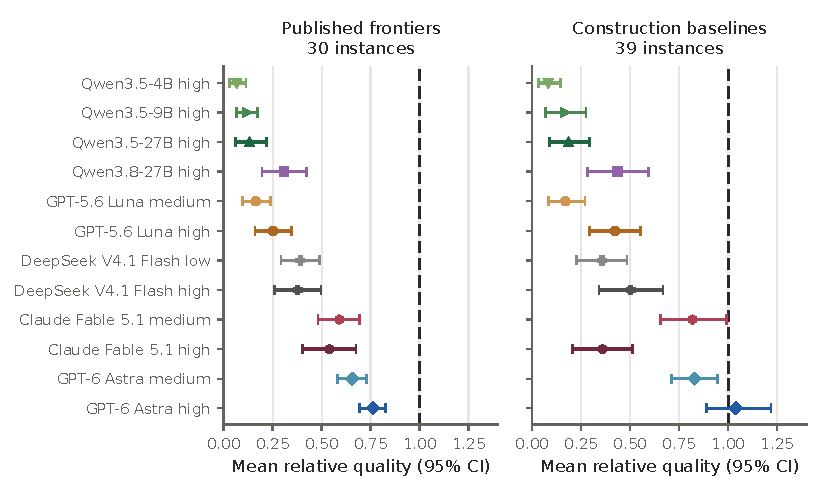
\includegraphics[width=\linewidth]{figs/fig2_headline.pdf}
\captionof{figure}{Fourteen-family construction quality for all twelve tool-free configurations. Whiskers show $95\%$ confidence intervals obtained by resampling instances within each reference group: 30 with published frontiers and 39 with construction baselines.}
\label{fig:headline}
\end{center}
The overall score in Table~\ref{tab:headline} combines all 69 instances using the definition in Section~\ref{sec:scoring}.
\appendixpage
\subsection{Performance across parameter ranges}
\readingnote{The non-code experiments use three parameter ranges: A1 contains small familiar instances, A2 uses larger settings, and A3 supplies the main evaluation. Family coverage varies across these groups. Appendix~\ref{app:ladder_results} instead varies size within each family, allowing construction quality to be followed as the task grows.}
\begin{center}
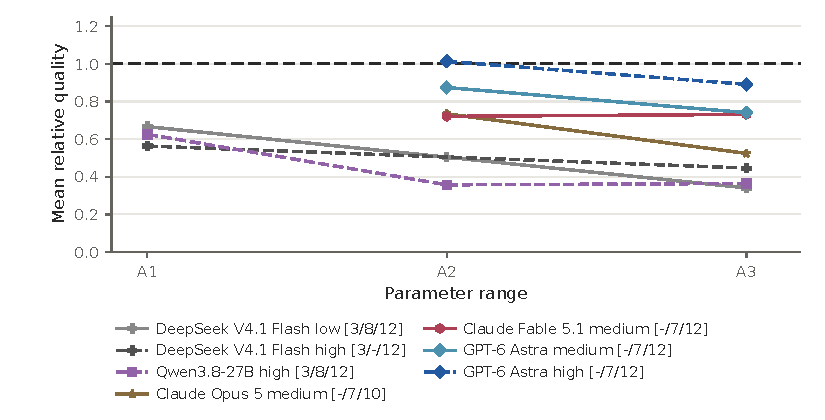
\includegraphics[width=\linewidth]{figs/fig3_tiers.pdf}
\captionof{figure}{Performance across parameter ranges. Legend brackets give the numbers of evaluated families in A1, A2 and A3, respectively; a dash denotes an unmeasured group. The family sets differ across groups.}
\label{fig:tiers}
\end{center}
\appendixpage
\subsection{Model size and reasoning effort}
\label{app:effort_results}
\readingnote{Qwen3.5's mean quality and validity increase across the three checkpoint sizes. The GPT-6 Astra experiment extends the reasoning-effort comparison to xhigh on shared smaller instances.}
On the main 69 instances, Astra medium and high return \AstraMedValidCalls{} and \AstraHighValidCalls{} valid constructions. To include xhigh effort, we also compare Astra on \AstraEffN{} shared smaller instances. Its mean relative quality is $\AstraMedATwoHFR$ at medium, $\AstraHighATwoHFR$ at high and $\AstraXhighATwoHFR$ at xhigh.
\begin{center}
\centering
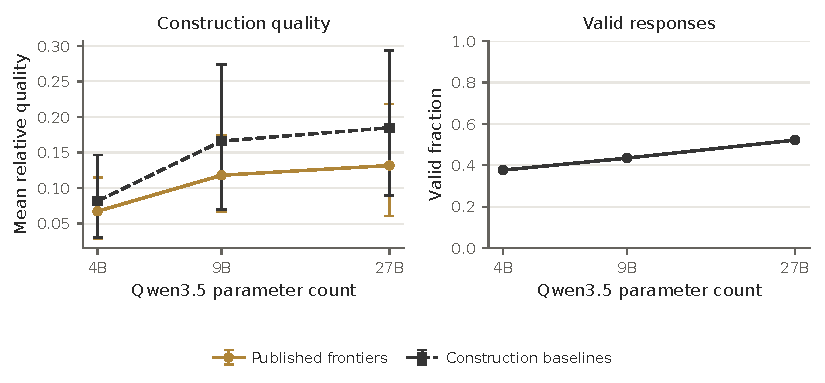
\includegraphics[width=\linewidth]{figs/fig7_model_size.pdf}
\captionof{figure}{Model-size comparison within Qwen3.5: 4B, 9B and 27B at high effort on the 69 instances. Left: mean relative quality with bootstrap CIs. Right: valid-response fraction. Model size varies while the problems remain fixed.}
\label{fig:model_size}
\end{center}
\begin{center}
\centering
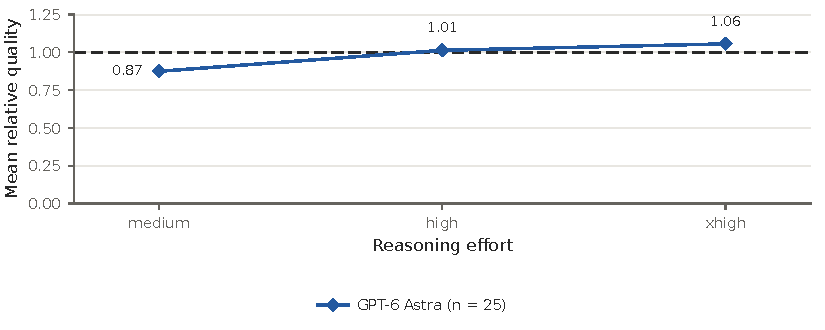
\includegraphics[width=\linewidth]{figs/fig4_effort.pdf}
\captionof{figure}{Mean relative quality for GPT-6 Astra at medium, high and xhigh effort on the same \AstraEffN{} smaller instances (A2). Multiple responses are averaged within each instance. All responses are valid at each effort level.}
\label{fig:effort}
\end{center}
\appendixpage
\subsection{Size--quality curves: cap sets, spherical codes and graphs}
\label{app:ladder_results}
\readingnote{Cap-set products allow GPT-6 Astra to retain quality at larger dimensions. Its graphs with maximum degree three remain valid while falling behind the reference as diameter increases. The lower panels apply the displayed transformations to construction sizes, showing how the model answers and references scale.}
\begin{center}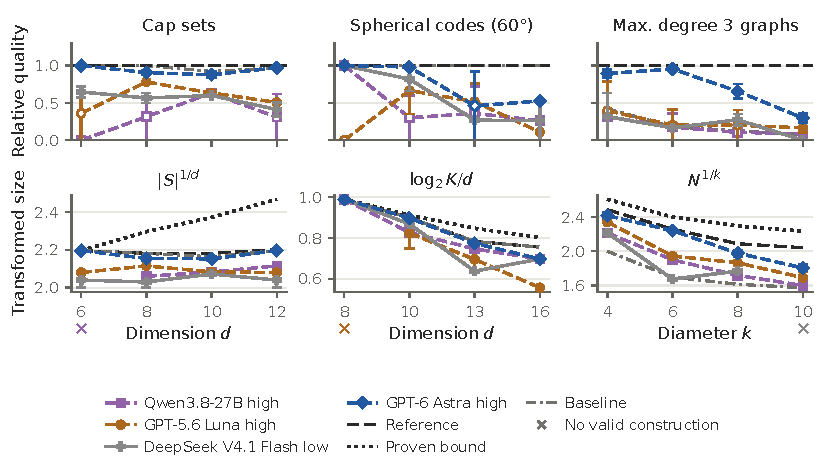
\includegraphics[width=\linewidth]{figs/fig6_ladder_main.pdf}
\captionof{figure}{Size--quality curves for cap sets, spherical codes and degree--diameter graphs. Upper panels average two independent responses per size, including zero scores; whiskers show their range and hollow markers indicate at least one invalid response. Lower panels use valid responses only; crosses below the axes mark sizes with no valid construction, using the model's colour. Transformations and line conventions follow Figure~\ref{fig:ladder}.}
\label{fig:ladder_first}
\end{center}
\appendixpage
\subsection{Size--quality curves: colourings, coverings and integer sets}
\readingnote{These curves vary the number of Schur colours, the size of the set covered by a design, and the integer interval from which a progression-free subset is chosen. The integer task supplements the five benchmark families in this experiment. The lower panels show the transformed construction sizes specified above each panel.}
\begin{center}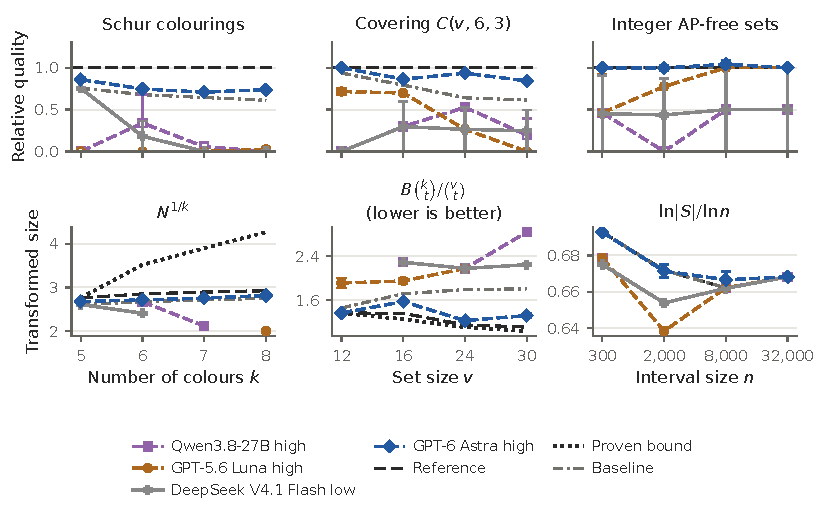
\includegraphics[width=\linewidth]{figs/appendix/ladder_designs.pdf}
\captionof{figure}{Size--quality curves for Schur colourings, covering designs and integer progression-free sets. Each size has two independent responses per configuration. Upper panels include zero scores; lower panels use valid answers. For Schur, $N$ is the largest coloured integer and $k$ the number of colours. For coverings, $B$ blocks of size $k$ cover every $t$-subset of a $v$-element set. For integer sets, $|S|$ elements are selected from $\{1,\ldots,n\}$. Whiskers show the range of the responses included in each panel.}
\label{fig:ladder_designs}
\end{center}
\appendixpage
\subsection{A changing reference: graphs with maximum degree four}
\readingnote{GPT-6 Astra's relative quality falls from \QuarticMTwo{} to \QuarticMFour{}. Its graph size changes from 192 to 195 vertices as the allowed diameter increases from five to seven, while the reference grows more quickly.}
\begin{center}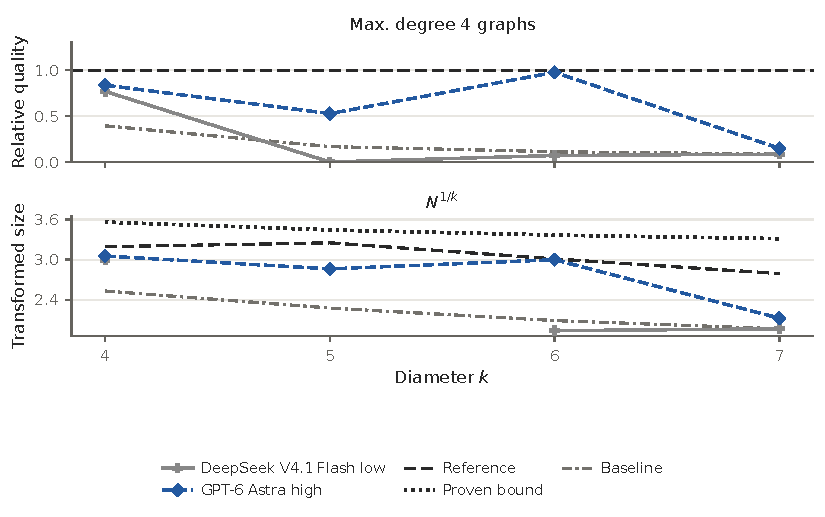
\includegraphics[width=\linewidth]{figs/appendix/ladder_quartic.pdf}
\captionof{figure}{Graphs with maximum degree four at diameters 4--7. The lower panel plots $N^{1/k}$, where $N$ is the number of vertices and $k$ the allowed diameter. Each point represents one response from GPT-6 Astra at high effort or DeepSeek V4.1 Flash at low effort.}
\label{fig:ladder_quartic}
\end{center}
\appendixpage
\subsection{Problem-size experiments: instances and references}
\small
\begin{longtable}{@{}P{.29\linewidth}P{.38\linewidth}rr@{}}
\caption{Problem-size experiments: instances and references. An asterisk marks a construction baseline.}\label{tab:ladder_parameters}\\
\toprule
Family & Parameters & Reference & Baseline \\
\midrule\endfirsthead
\toprule
Family & Parameters & Reference & Baseline \\
\midrule\endhead
\bottomrule\endfoot
cap set & d=6 & 112 & 112 \\
cap set & d=8 & 512 & 512 \\
cap set & d=10 & 2432 & 2240 \\
cap set & d=12 & 12928 & 12544 \\
spherical codes ($60^\circ$) & d=8 & 240 & 240 \\
spherical codes ($60^\circ$) & d=10 & 510 & 510 \\
spherical codes ($60^\circ$) & d=13 & 1154 & 1154 \\
spherical codes ($60^\circ$) & d=16 & 4320 & 4320 \\
max. degree 3 graphs & d=3, k=4 & 38 & 16 \\
max. degree 3 graphs & d=3, k=6 & 132 & 24 \\
max. degree 3 graphs & d=3, k=8 & 360 & 46 \\
max. degree 3 graphs & d=3, k=10 & 1250 & 94 \\
Schur & k=5 & 160 & 121 \\
Schur & k=6 & 536 & 364 \\
Schur & k=7 & 1696 & 1093 \\
Schur & k=8 & 5362 & 3280 \\
covering & v=12, k=6, t=3 & 15 & 16 \\
covering & v=16, k=6, t=3 & 38 & 48 \\
covering & v=24, k=6, t=3 & 116 & 181 \\
covering & v=30, k=6, t=3 & 225 & 366 \\
max. degree 4 graphs & d=4, k=4 & 104 & 41 \\
max. degree 4 graphs & d=4, k=5 & 364 & 61 \\
max. degree 4 graphs & d=4, k=6 & 745 & 83 \\
max. degree 4 graphs & d=4, k=7 & 1320 & 113 \\
integer AP-free sets & k=3, n=300 & 52* & 52 \\
integer AP-free sets & k=3, n=2000 & 165* & 165 \\
integer AP-free sets & k=3, n=8000 & 384* & 384 \\
integer AP-free sets & k=3, n=32000 & 1024* & 1024 \\
\end{longtable}

\normalsize
\appendixpage
\subsection{Problem-size experiments: relative quality}
\small\setlength{\tabcolsep}{2pt}
\begin{longtable}{@{}P{.23\linewidth}lrrrr@{}}
\caption{Mean relative quality at each problem size. Parentheses give valid responses out of the total; means include zero scores.}\label{tab:ladder}\\
\toprule
Family & Size & \shortstack{Qwen3.8-27B\\high} & \shortstack{GPT-5.6 Luna\\high} & \shortstack{DeepSeek V4.1\\Flash low} & \shortstack{GPT-6 Astra\\high} \\
\midrule\endfirsthead
\toprule
Family & Size & \shortstack{Qwen3.8-27B\\high} & \shortstack{GPT-5.6 Luna\\high} & \shortstack{DeepSeek V4.1\\Flash low} & \shortstack{GPT-6 Astra\\high} \\
\midrule\endhead
\bottomrule\endfoot
cap set & $d=6$ & 0.00 (0/2) & 0.36 (1/2) & 0.65 (2/2) & 1.00 (2/2) \\
cap set & $d=8$ & 0.32 (1/2) & 0.78 (2/2) & 0.57 (2/2) & 0.91 (2/2) \\
cap set & $d=10$ & 0.63 (2/2) & 0.63 (2/2) & 0.60 (2/2) & 0.88 (2/2) \\
cap set & $d=12$ & 0.31 (1/2) & 0.51 (2/2) & 0.41 (2/2) & 0.97 (2/2) \\
spherical codes ($60^\circ$) & $d=8$ & 1.00 (2/2) & 0.00 (0/2) & 1.00 (2/2) & 1.00 (2/2) \\
spherical codes ($60^\circ$) & $d=10$ & 0.30 (1/2) & 0.67 (2/2) & 0.82 (2/2) & 0.98 (2/2) \\
spherical codes ($60^\circ$) & $d=13$ & 0.36 (1/2) & 0.52 (2/2) & 0.27 (2/2) & 0.46 (1/2) \\
spherical codes ($60^\circ$) & $d=16$ & 0.26 (1/2) & 0.11 (2/2) & 0.26 (1/2) & 0.53 (2/2) \\
max. degree 3 graphs & $k=4$ & 0.32 (1/2) & 0.39 (1/2) & 0.32 (1/2) & 0.89 (2/2) \\
max. degree 3 graphs & $k=6$ & 0.18 (1/2) & 0.20 (1/2) & 0.17 (2/2) & 0.95 (2/2) \\
max. degree 3 graphs & $k=8$ & 0.11 (1/2) & 0.20 (1/2) & 0.28 (2/2) & 0.66 (2/2) \\
max. degree 3 graphs & $k=10$ & 0.09 (2/2) & 0.17 (2/2) & 0.00 (0/2) & 0.30 (2/2) \\
Schur & $k=5$ & 0.00 (0/2) & 0.00 (0/2) & 0.76 (2/2) & 0.86 (2/2) \\
Schur & $k=6$ & 0.34 (1/2) & 0.00 (0/2) & 0.18 (1/2) & 0.75 (2/2) \\
Schur & $k=7$ & 0.06 (1/2) & 0.00 (0/2) & 0.00 (0/2) & 0.71 (2/2) \\
Schur & $k=8$ & 0.00 (0/2) & 0.02 (1/2) & 0.00 (0/2) & 0.74 (2/2) \\
covering & $v=12$ & 0.00 (0/2) & 0.72 (2/2) & 0.00 (0/2) & 1.00 (2/2) \\
covering & $v=16$ & 0.30 (1/2) & 0.70 (2/2) & 0.30 (1/2) & 0.86 (2/2) \\
covering & $v=24$ & 0.53 (2/2) & 0.26 (1/2) & 0.26 (1/2) & 0.94 (2/2) \\
covering & $v=30$ & 0.20 (1/2) & 0.00 (0/2) & 0.25 (1/2) & 0.84 (2/2) \\
max. degree 4 graphs & $k=4$ & -- & -- & 0.77 (1/1) & 0.84 (1/1) \\
max. degree 4 graphs & $k=5$ & -- & -- & 0.00 (0/1) & 0.53 (1/1) \\
max. degree 4 graphs & $k=6$ & -- & -- & 0.07 (1/1) & 0.98 (1/1) \\
max. degree 4 graphs & $k=7$ & -- & -- & 0.09 (1/1) & 0.15 (1/1) \\
integer AP-free sets & $n=300$ & 0.46 (1/2) & 0.46 (1/2) & 0.45 (1/2) & 1.00 (2/2) \\
integer AP-free sets & $n=2000$ & 0.00 (0/2) & 0.78 (2/2) & 0.44 (1/2) & 1.00 (2/2) \\
integer AP-free sets & $n=8000$ & 0.50 (1/2) & 1.00 (2/2) & 0.50 (1/2) & 1.04 (2/2) \\
integer AP-free sets & $n=32000$ & 0.50 (1/2) & 1.00 (2/2) & 0.50 (1/2) & 1.00 (2/2) \\
\end{longtable}

\normalsize
\appendixpage
\subsection{Code quality across increasing lengths}
\readingnote{The same finite factors can generate large Shannon products, while trifference certificates represent codes far beyond an explicit list. Relative quality measures their quality at each length. The lower panels express code size $M$ as a per-coordinate growth base $M^{1/d}$ for Shannon and a ternary rate $\log_3 M/n$ for trifference, where $d$ and $n$ are codeword lengths.}
\begin{center}
\centering
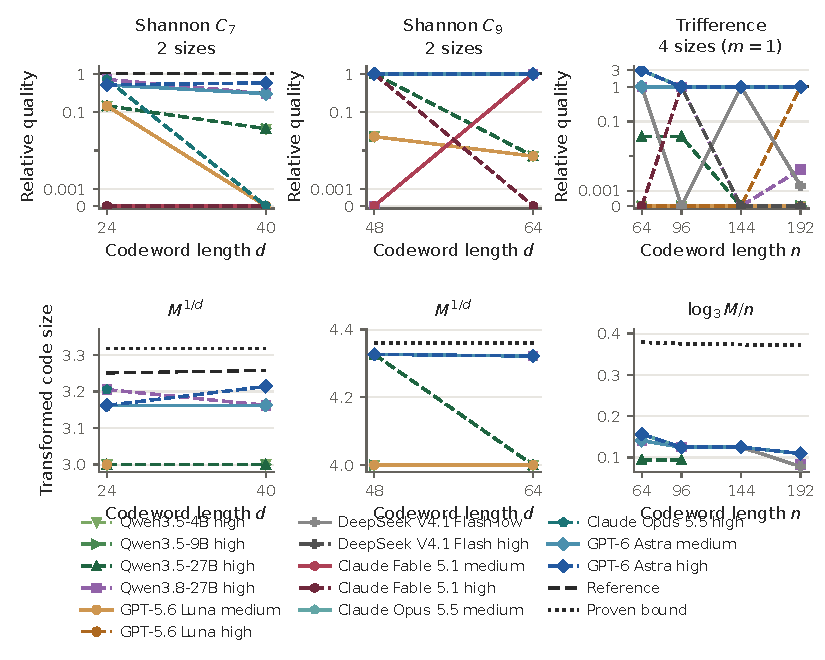
\includegraphics[width=\linewidth]{figs/fig8_code_scale.pdf}
\captionof{figure}{Code-family size--quality curves for all twelve configurations. Top: relative quality, including zero scores. Bottom: per-coordinate growth for Shannon and ternary rate for trifference, using valid answers only; missing points break the curves. Dark dashed lines are references; dark dotted lines are proven upper bounds. Shannon has two codeword lengths per cycle size; trifference has four lengths at $m=1$. Each point represents one response.}
\label{fig:code_scale}
\end{center}
\appendixpage
\subsection{Code-family results}
\label{app:code_comparison}
Table~\ref{tab:code_comparison} compares all twelve tool-free configurations on four Shannon and four trifference instances. Appendix~\ref{case:shannon} gives the Shannon product construction and its verification.
\begin{center}\footnotesize\setlength{\tabcolsep}{3pt}
\begin{tabular}{@{}lrrrrr@{}}
\toprule
configuration & \shortstack{Shannon\\relative quality} & valid & \shortstack{Trifference\\relative quality} & valid & words at $n=192$ \\
\midrule
Qwen3.5-4B high & 0.053 & 4/4 & 0.000 & 0/4 & 0 \\
Qwen3.5-9B high & 0.053 & 4/4 & 0.000 & 0/4 & 0 \\
Qwen3.5-27B high & 0.297 & 4/4 & 0.019 & 2/4 & 0 \\
Qwen3.8-27B high & 0.504 & 3/4 & 0.501 & 3/4 & $4.30\times10^{7}$ \\
GPT-5.6 Luna medium & 0.044 & 3/4 & 0.000 & 0/4 & 0 \\
GPT-5.6 Luna high & 0.705 & 4/4 & 0.250 & 1/4 & $1.05\times10^{10}$ \\
DeepSeek V4.1 Flash low & 0.705 & 4/4 & 0.500 & 3/4 & $1.43\times10^{7}$ \\
DeepSeek V4.1 Flash high & 0.705 & 4/4 & 0.250 & 1/4 & 0 \\
Claude Fable 5.1 medium & 0.250 & 1/4 & 1.000 & 4/4 & $1.05\times10^{10}$ \\
Claude Fable 5.1 high & 0.250 & 1/4 & 0.750 & 3/4 & $1.05\times10^{10}$ \\
Claude Opus 5.5 medium & 0.705 & 4/4 & 1.500 & 4/4 & $1.05\times10^{10}$ \\
Claude Opus 5.5 high & 0.678 & 3/4 & 1.500 & 4/4 & $1.05\times10^{10}$ \\
GPT-6 Astra medium & 0.705 & 4/4 & 1.000 & 4/4 & $1.05\times10^{10}$ \\
GPT-6 Astra high & 0.774 & 4/4 & 1.500 & 4/4 & $1.05\times10^{10}$ \\
\bottomrule
\end{tabular}

\captionof{table}{Tool-free code-family results on four instances per family, including zero scores. A ratio of $1$ matches the construction baseline. The last column gives the trifference code size at length 192, or zero for failure.}
\label{tab:code_comparison}
\end{center}

For trifference, GPT-6 Astra at high effort without tools produces 59,049 codewords at length 64, three times the baseline, and matches the construction baseline at the other three lengths. Astra medium and Claude Fable 5.1 medium match the baselines at all four lengths, certifying $3^{21}$ codewords at length 192. GPT-5.6 Luna at medium effort has no valid trifference answer, while Luna high matches the baseline only at length 192. Figure~\ref{fig:code_scale} shows how code size scales with length and compares the results with the references and proven bounds.

\appendixpage
Tables~\ref{tab:code_multimodel_detail} and \ref{tab:code_detail_trifference} give the individual outcomes behind these averages.
\begin{center}\small\setlength{\tabcolsep}{5pt}
\begin{tabularx}{\linewidth}{@{}Xrrrr@{}}
\toprule
Model / effort & $(7,24)$ & $(7,40)$ & $(9,48)$ & $(9,64)$ \\
\midrule
Qwen3.5-4B high & 0.145 & 0.037 & 0.023 & 0.007 \\
Qwen3.5-9B high & 0.145 & 0.037 & 0.023 & 0.007 \\
Qwen3.5-27B high & 0.145 & 0.037 & 1.000 & 0.007 \\
Qwen3.8-27B high & 0.713 & 0.304 & 0.000$^{\dagger}$ & 1.000 \\
GPT-5.6 Luna medium & 0.145 & 0.000$^{\dagger}$ & 0.023 & 0.007 \\
GPT-5.6 Luna high & 0.515 & 0.304 & 1.000 & 1.000 \\
DeepSeek V4.1 Flash low & 0.515 & 0.304 & 1.000 & 1.000 \\
DeepSeek V4.1 Flash high & 0.515 & 0.304 & 1.000 & 1.000 \\
Claude Fable 5.1 medium & 0.000$^{\dagger}$ & 0.000$^{\dagger}$ & 0.000$^{\dagger}$ & 1.000 \\
Claude Fable 5.1 high & 0.000$^{\dagger}$ & 0.000$^{\dagger}$ & 1.000 & 0.000$^{\dagger}$ \\
GPT-6 Astra medium & 0.515 & 0.304 & 1.000 & 1.000 \\
GPT-6 Astra high & 0.515 & 0.582 & 1.000 & 1.000 \\
\bottomrule
\end{tabularx}

\captionof{table}{Shannon relative quality on the four evaluated instances. A dagger marks an invalid or budget-exhausted response, scored zero.}
\label{tab:code_multimodel_detail}
\end{center}
\begin{center}\small\setlength{\tabcolsep}{5pt}
\begin{tabularx}{\linewidth}{@{}Xrrrr@{}}
\toprule
Model / effort & 64 & 96 & 144 & 192 \\
\midrule
Qwen3.5-4B high & 0.000$^{\dagger}$ & 0.000$^{\dagger}$ & 0.000$^{\dagger}$ & 0.000$^{\dagger}$ \\
Qwen3.5-9B high & 0.000$^{\dagger}$ & 0.000$^{\dagger}$ & 0.000$^{\dagger}$ & 0.000$^{\dagger}$ \\
Qwen3.5-27B high & 0.037 & 0.037 & 0.000$^{\dagger}$ & 0.000$^{\dagger}$ \\
Qwen3.8-27B high & 1.000 & 1.000 & 0.000$^{\dagger}$ & 0.004 \\
GPT-5.6 Luna medium & 0.000$^{\dagger}$ & 0.000$^{\dagger}$ & 0.000$^{\dagger}$ & 0.000$^{\dagger}$ \\
GPT-5.6 Luna high & 0.000$^{\dagger}$ & 0.000$^{\dagger}$ & 0.000$^{\dagger}$ & 1.000 \\
DeepSeek V4.1 Flash low & 1.000 & 0.000$^{\dagger}$ & 1.000 & 0.001 \\
DeepSeek V4.1 Flash high & 0.000$^{\dagger}$ & 1.000 & 0.000$^{\dagger}$ & 0.000$^{\dagger}$ \\
Claude Fable 5.1 medium & 1.000 & 1.000 & 1.000 & 1.000 \\
Claude Fable 5.1 high & 0.000$^{\dagger}$ & 1.000 & 1.000 & 1.000 \\
Claude Opus 5.5 medium & 3.000 & 1.000 & 1.000 & 1.000 \\
Claude Opus 5.5 high & 3.000 & 1.000 & 1.000 & 1.000 \\
GPT-6 Astra medium & 1.000 & 1.000 & 1.000 & 1.000 \\
GPT-6 Astra high & 3.000 & 1.000 & 1.000 & 1.000 \\
\bottomrule
\end{tabularx}

\captionof{table}{Trifference relative quality at separation multiplicity $m=1$. A dagger marks an invalid or budget-exhausted response, scored zero.}
\label{tab:code_detail_trifference}
\end{center}
\appendixpage
\subsection{Failures and answer formats}
Zero-score responses arise from invalid mathematical constructions, malformed descriptions, or empty and budget-exhausted answers, with the reason for each response recorded in the released data. A format error can obscure a valid construction, as in DeepSeek V4.1 Flash's length-96 trifference response at low effort, which supplies generator rows as integer arrays rather than the required digit strings. Expressing those rows in the required format gives a valid 19,683-word code, although the reported score uses the submitted representation.

\subsection{Smaller trifference instances}
\label{app:codes}
Four smaller trifference instances test the quality of finite codes that can serve as ingredients for larger constructions. Table~\ref{tab:codes} evaluates GPT-6 Astra at medium effort on $(n,m)=(30,1),(36,2),(42,3),(56,1)$, complementing the larger instances in the main evaluation.

Astra matches the construction baselines at lengths 30, 36 and 42 with valid 729-word codes, and triples the reference at length 56 with a 6,561-word code. These finite constructions can be represented explicitly, while algebraic certificates (Appendix~\ref{app:trifference_certificates}) extend evaluation to larger codes whose words cannot all be listed within a response.
\begin{center}\begin{minipage}{\linewidth}\centering\small
\begin{tabular}{@{}rrrrrc@{}}
\toprule
Length $n$ & Separation $m$ & Reference & Model & \shortstack{Relative\\quality} & Valid \\
\midrule
30 & 1 & 729 & 729 & 1.000 & yes \\
36 & 2 & 729 & 729 & 1.000 & yes \\
42 & 3 & 729 & 729 & 1.000 & yes \\
56 & 1 & 2187 & 6561 & 3.000 & yes \\
\bottomrule
\end{tabular}
\captionof{table}{GPT-6 Astra at medium effort on four smaller trifference instances. Code sizes are compared with construction baselines.}
\label{tab:codes}
\end{minipage}\end{center}

\appendixpage
\subsection{Claude Opus 5 on shared instances}
\label{app:opus_subset}
Claude Opus 5 at medium effort is compared with the other configurations on their 45 shared instances.
\begin{center}
\centering\footnotesize
\begin{tabular}{@{}lrrrr@{}}
\toprule
& & \multicolumn{2}{c}{Mean relative quality} & \\
\cmidrule(lr){3-4}
configuration & \shortstack{Overall\\score} & \shortstack{Published\\frontiers (15)} & \shortstack{Construction\\baselines (30)} & \shortstack{Valid\\fraction} \\
\midrule
Claude Opus 5 medium & 52.41 & 0.48 & 0.55 & 0.87 \\
Qwen3.5-4B high & 7.69 & 0.08 & 0.07 & 0.38 \\
Qwen3.5-9B high & 16.96 & 0.14 & 0.18 & 0.47 \\
Qwen3.5-27B high & 17.07 & 0.17 & 0.17 & 0.53 \\
Qwen3.8-27B high & 40.98 & 0.37 & 0.43 & 0.64 \\
GPT-5.6 Luna medium & 20.36 & 0.18 & 0.21 & 0.64 \\
GPT-5.6 Luna high & 32.77 & 0.23 & 0.37 & 0.71 \\
DeepSeek V4.1 Flash low & 34.30 & 0.43 & 0.30 & 0.80 \\
DeepSeek V4.1 Flash high & 45.40 & 0.34 & 0.51 & 0.78 \\
Claude Fable 5.1 medium & 75.64 & 0.54 & 0.86 & 0.87 \\
Claude Fable 5.1 high & 36.89 & 0.54 & 0.29 & 0.44 \\
Claude Opus 5.5 medium & 60.16 & 0.58 & 0.61 & 0.87 \\
Claude Opus 5.5 high & 71.38 & 0.72 & 0.71 & 0.87 \\
GPT-6 Astra medium & 74.57 & 0.60 & 0.82 & 0.98 \\
GPT-6 Astra high & 91.48 & 0.74 & 1.00 & 1.00 \\
\bottomrule
\end{tabular}

\captionof{table}{Comparison with Claude Opus 5 at medium effort on 45 shared instances: 15 with published frontiers and 30 with construction baselines. The overall score is 100 times the mean relative quality over this subset.}
\label{tab:opus_subset}
\end{center}
\subsection{Sensitivity to family selection}
\label{app:selection}
We examine the effect of including Kakeya as a scored family in Table~\ref{tab:selection}. This comparison uses the twelve non-code families, with and without Kakeya, on identical model responses. Spherical-code variants share one family label, as do the two Heilbronn domains; each distinct task and parameter setting retains equal weight. Kakeya affects only the mean relative quality on instances with construction baselines and the mean gap closed, leaving the published-frontier results unchanged.
\begin{center}
\centering\footnotesize
\resizebox{\linewidth}{!}{\begin{tabular}{@{}lrrrr@{}}
\toprule
configuration & \shortstack{Relative quality\\$+K$} & \shortstack{Relative quality\\$-K$} & \shortstack{Gap closed\\$+K$} & \shortstack{Gap closed\\$-K$} \\
\midrule
Qwen3.5-4B high & 0.088 & 0.096 & 0.000 & 0.000 \\
Qwen3.5-9B high & 0.191 & 0.202 & 0.000 & 0.000 \\
Qwen3.5-27B high & 0.184 & 0.192 & 0.000 & 0.000 \\
Qwen3.8-27B high & 0.425 & 0.418 & 0.005 & 0.004 \\
GPT-5.6 Luna medium & 0.203 & 0.207 & 0.000 & 0.000 \\
GPT-5.6 Luna high & 0.419 & 0.408 & 0.002 & 0.002 \\
DeepSeek V4.1 Flash low & 0.283 & 0.292 & 0.000 & 0.000 \\
DeepSeek V4.1 Flash high & 0.470 & 0.510 & 0.006 & 0.007 \\
Claude Fable 5.1 medium & 0.880 & 0.868 & 0.013 & 0.014 \\
GPT-6 Astra medium & 0.838 & 0.822 & 0.006 & 0.007 \\
GPT-6 Astra high & 1.015 & 1.014 & 0.017 & 0.017 \\
\bottomrule
\end{tabular}
}
\captionof{table}{Effect of including Kakeya in the aggregate. $+K$ includes Kakeya and $-K$ excludes it. Relative quality is averaged over instances with construction baselines; both settings use the same responses from the twelve non-code families and equal instance weights. Published-frontier scores are identical in the two cases.}
\label{tab:selection}
\end{center}

\appendixpage
\subsection{Gap closed and progress toward the LABS target}
\label{app:gap_breakdown}
Gap closed starts at the same reference as relative quality and measures logarithmic progress toward a proven bound. Table~\ref{tab:gap_breakdown} separates the two reference groups. The combined value gives each eligible instance equal weight, so the groups contribute in proportion to their 30 and 34 instances. Invalid answers and valid answers that do not exceed the reference contribute zero.

The five LABS instances instead use the conjectured merit-factor target of 12.32. We compute progress from each construction baseline toward this target using the same logarithmic formula, and report it separately. These five values do not enter the proven-bound mean in Table~\ref{tab:headline}.
\begin{center}
\footnotesize\setlength{\tabcolsep}{4pt}
\begin{tabular}{@{}lrrrr@{}}
\toprule
& \multicolumn{3}{c}{Gap closed to proven bounds} & LABS target \\
\cmidrule(lr){2-4}
Configuration & All 64 & Published 30 & Construction 34 & 5 instances \\
\midrule
Qwen3.5-4B high & 0.000 & 0.000 & 0.000 & 0.000 \\
Qwen3.5-9B high & 0.000 & 0.000 & 0.000 & 0.000 \\
Qwen3.5-27B high & 0.000 & 0.000 & 0.000 & 0.000 \\
Qwen3.8-27B high & 0.004 & 0.000 & 0.007 & 0.000 \\
GPT-5.6 Luna medium & 0.000 & 0.000 & 0.000 & 0.000 \\
GPT-5.6 Luna high & 0.002 & 0.000 & 0.004 & 0.000 \\
DeepSeek V4.1 Flash low & 0.000 & 0.000 & 0.000 & 0.000 \\
DeepSeek V4.1 Flash high & 0.006 & 0.000 & 0.011 & 0.000 \\
Claude Fable 5.1 medium & 0.012 & 0.000 & 0.023 & 0.000 \\
Claude Fable 5.1 high & 0.003 & 0.000 & 0.006 & 0.000 \\
GPT-6 Astra medium & 0.006 & 0.000 & 0.011 & 0.000 \\
GPT-6 Astra high & 0.016 & 0.000 & 0.030 & 0.006 \\
\midrule
GPT-6 Astra high + tools & 0.063 & 0.000 & 0.118 & 0.401 \\
GPT-5.6 Luna high + tools & 0.047 & 0.000 & 0.088 & 0.247 \\
\bottomrule
\end{tabular}

\captionof{table}{Mean progress from the reference. The first three numeric columns use proven mathematical bounds; the last uses the conjectured LABS target. Each mean includes zero scores.}
\label{tab:gap_breakdown}
\end{center}
